% TODO: links in ecosystem models
% TODO: deeper XNN case study

\documentclass[11pt,aspectratio=169,hyperref={colorlinks}]{beamer}

\usetheme{Singapore}

\usecolortheme[snowy]{owl}

\usepackage[utf8]{inputenc}
\usepackage[T1]{fontenc}
\usepackage[american]{babel}
\usepackage{graphicx}
\usepackage{hyperref}
\hypersetup{
    colorlinks=true,
    urlcolor=[rgb]{0,0,0.61},
    linkcolor=[rgb]{0,0,0.61}}
\usepackage[natbib=true,style=authoryear,backend=bibtex,useprefix=true]{biblatex}
\usepackage{blindtext}

%-------------------------------------------------------------------------------

\usepackage{mathtools}
\usepackage{xcolor}
\usepackage{soul}
\newcommand{\mathcolorbox}[2]{\colorbox{#1}{$\displaystyle #2$}}

%-------------------------------------------------------------------------------

% OwlGreen - customized to make the header violet color
\definecolor{OwlGreen}{RGB}{51, 0, 102}

%-------------------------------------------------------------------------------

\setbeamertemplate{bibliography item}{}
\renewcommand*{\bibfont}{\scriptsize}
\addbibresource{lecture_1.bib}

\setbeamerfont{caption}{size=\footnotesize}
\setbeamertemplate{frametitle continuation}{}
\setcounter{tocdepth}{1}

%-------------------------------------------------------------------------------

\usenavigationsymbolstemplate{}
\setbeamertemplate{footline}{%
    \raisebox{5pt}{\makebox{\hfill\makebox[20pt]{\color{gray}
          \scriptsize\insertframenumber}}}\hspace*{5pt}}

\renewcommand*{\thefootnote}{\fnsymbol{footnote}}

%-------------------------------------------------------------------------------

\usepackage{epigraph}
% \epigraphsize{\small}% Default
\setlength\epigraphwidth{14cm}
\setlength\epigraphrule{0pt}
\usepackage{etoolbox}
\makeatletter
\patchcmd{\epigraph}{\@epitext{#1}}{\itshape\@epitext{#1}}{}{}
\makeatother

%-------------------------------------------------------------------------------

\author{Patrick Hall}
\title{Introduction to Responsible Machine Learning\footnote{\tiny{This material is shared under a \href{https://creativecommons.org/licenses/by/4.0/deed.ast}{CC By 4.0 license} which allows for editing and redistribution, even for commercial purposes. However, any derivative work should attribute the author.}}}
\subtitle{Lecture 1: Interpretable Machine Learning Models}
\institute{The George Washington University}
\date{\today}

%-------------------------------------------------------------------------------

\begin{document}
	
	\maketitle
	
	\begin{frame}
	
		\frametitle{Contents}
		
		\tableofcontents{}
		
	\end{frame}
	

%-------------------------------------------------------------------------------
	\section{Class Overview}
%-------------------------------------------------------------------------------	
	\subsection*{}
	
	\begin{frame}
	
		\frametitle{Grading and Policy}
			
		\begin{itemize}
			\item{Grading:}
				\begin{itemize}
					\item{$\frac{1}{3}$ Participation}
					\item{$\frac{1}{3}$ Project GitHub or Kaggle kernel}
                    \item{$\frac{1}{3}$ Public Kaggle leaderboard score}
				\end{itemize}
			\item{Project:}	
				\begin{itemize}
					\item{Kaggle competition using techniques from class}
					\item{Individual or group (no more than 4 members)}
					\item Select team members ASAP
				\end{itemize}
			\item \href{https://github.com/jphall663/GWU_rml/blob/master/rml_syllabus_summer_2020.pdf}{Syllabus}
			\item{Webex office hours: Thurs. 5-6 pm or by appointment}
			\item{Class resources: \url{https://jphall663.github.io/GWU_rml/}}	
		\end{itemize}		
			
	\end{frame}
	
	
	\begin{frame}
	
		\frametitle{Overview}
		
		\begin{itemize}
			\item{\textbf{Class 1}: Interpretable Models}
			\item{\textbf{Class 2}: Post-hoc Explanations}
			\item{\textbf{Class 3}: Fairness}
			\item{\textbf{Class 4}: Security}
			\item{\textbf{Class 5}: Model Debugging}
			\item{\textbf{Class 6}: Best Practices}
		\end{itemize}
			
					
	\end{frame}

%-------------------------------------------------------------------------------
	\section{Introduction}
%-------------------------------------------------------------------------------
	
		\subsection*{}

		\begin{frame}
	
			\frametitle{Responsible Artificial Intelligence}
	
			\epigraph{“Responsible Artificial Intelligence is about human responsibility for the development of intelligent systems along fundamental human principles and values, to ensure human-flourishing and well-being in a sustainable world.”}{--- \textup{Virginia Dignum}, \textbf{Responsible Artificial Intelligence}}
	
		\end{frame}		

		\begin{frame}
	
			\frametitle{What About Machine Learning?}
			
			\begin{figure}[htb]
				\begin{center}
					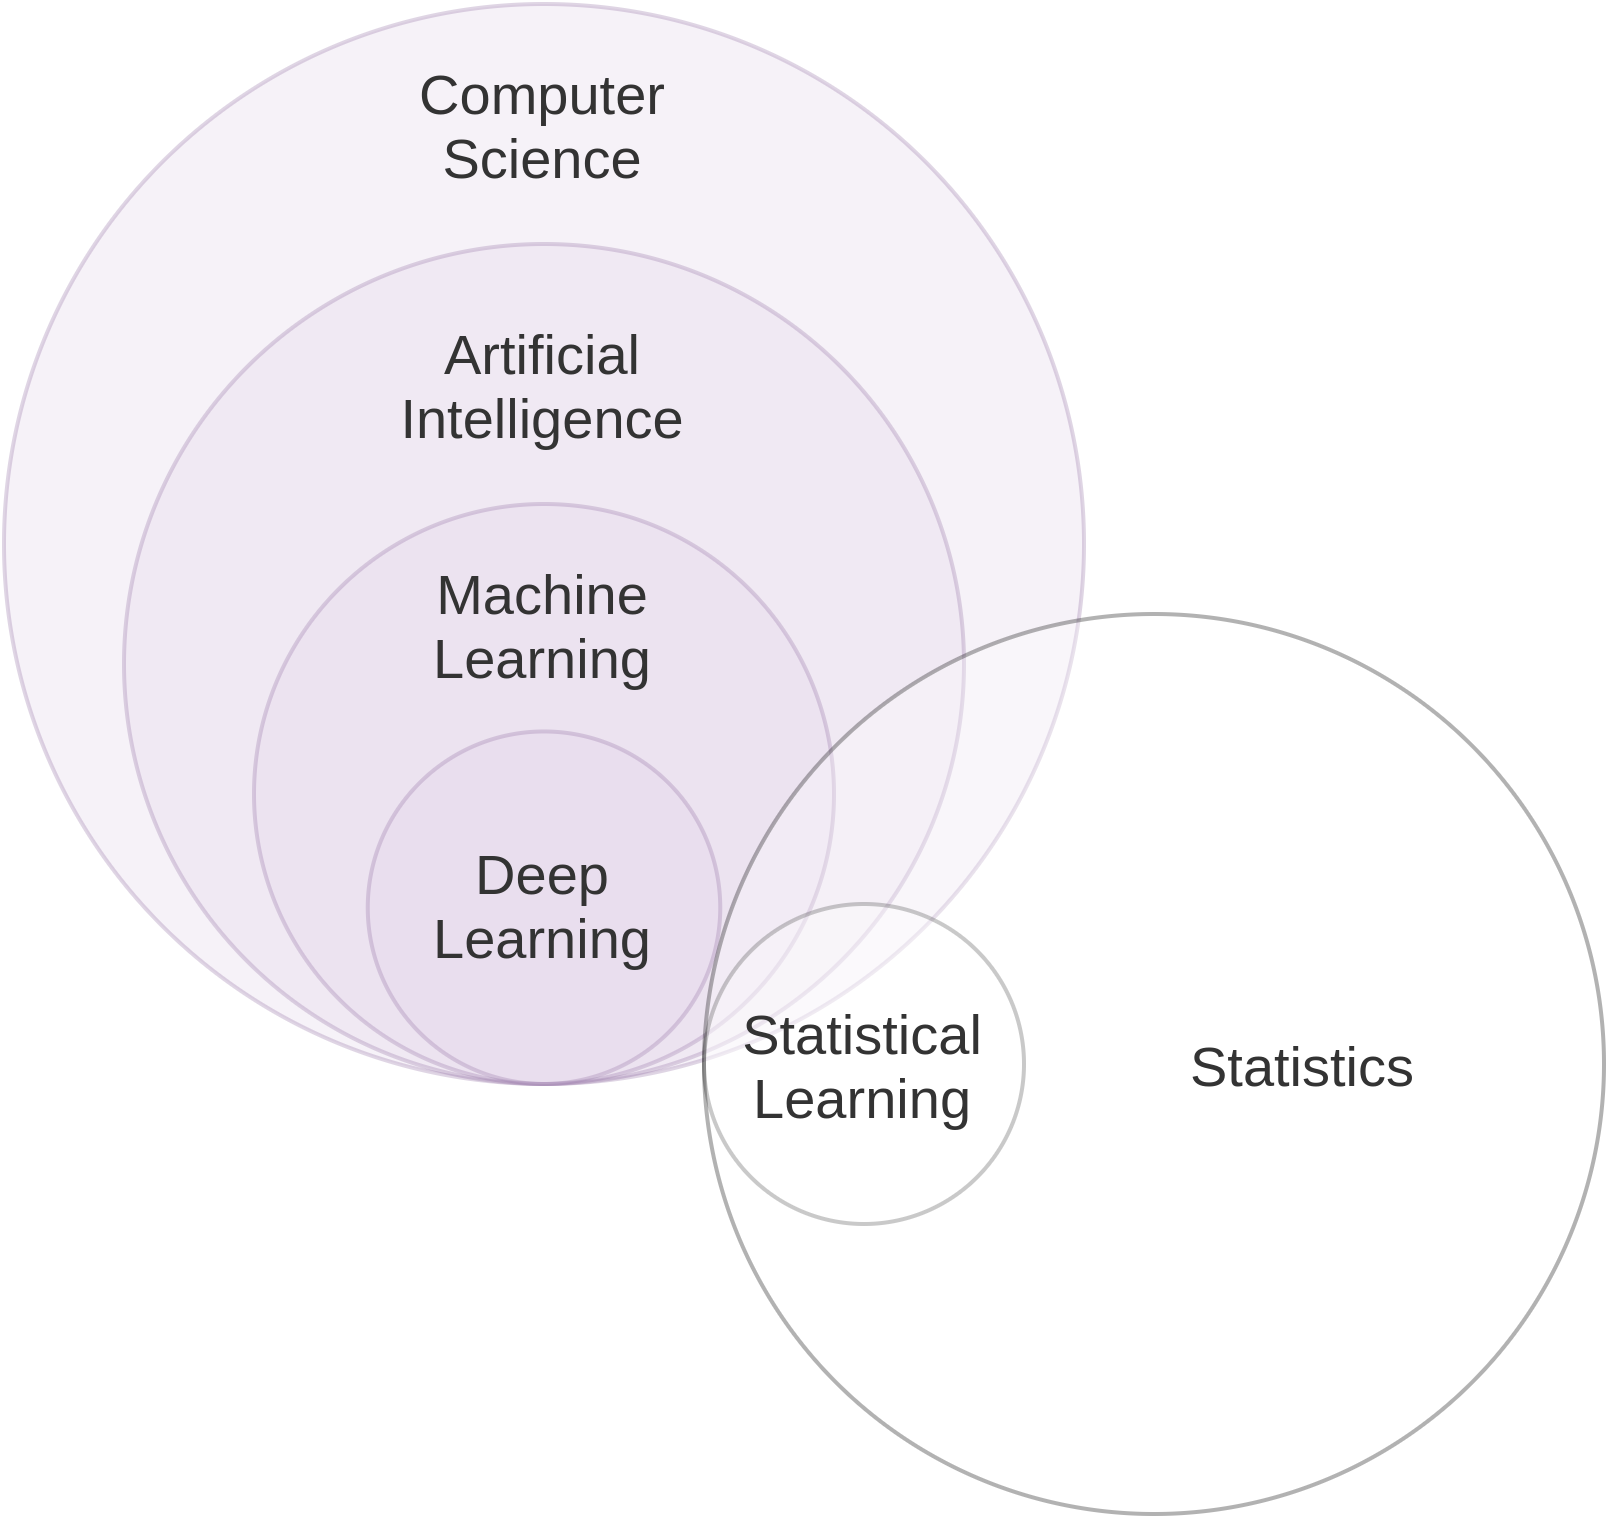
\includegraphics[height=150pt]{../img/cs_stat.png}
					\label{fig:cs_stat}
				\end{center}
			\end{figure}		
			
		\end{frame}	

		\begin{frame}
		
			\frametitle{A Responsible Machine Learning Workflow}
			
			\begin{figure}[htb]
				\begin{center}
					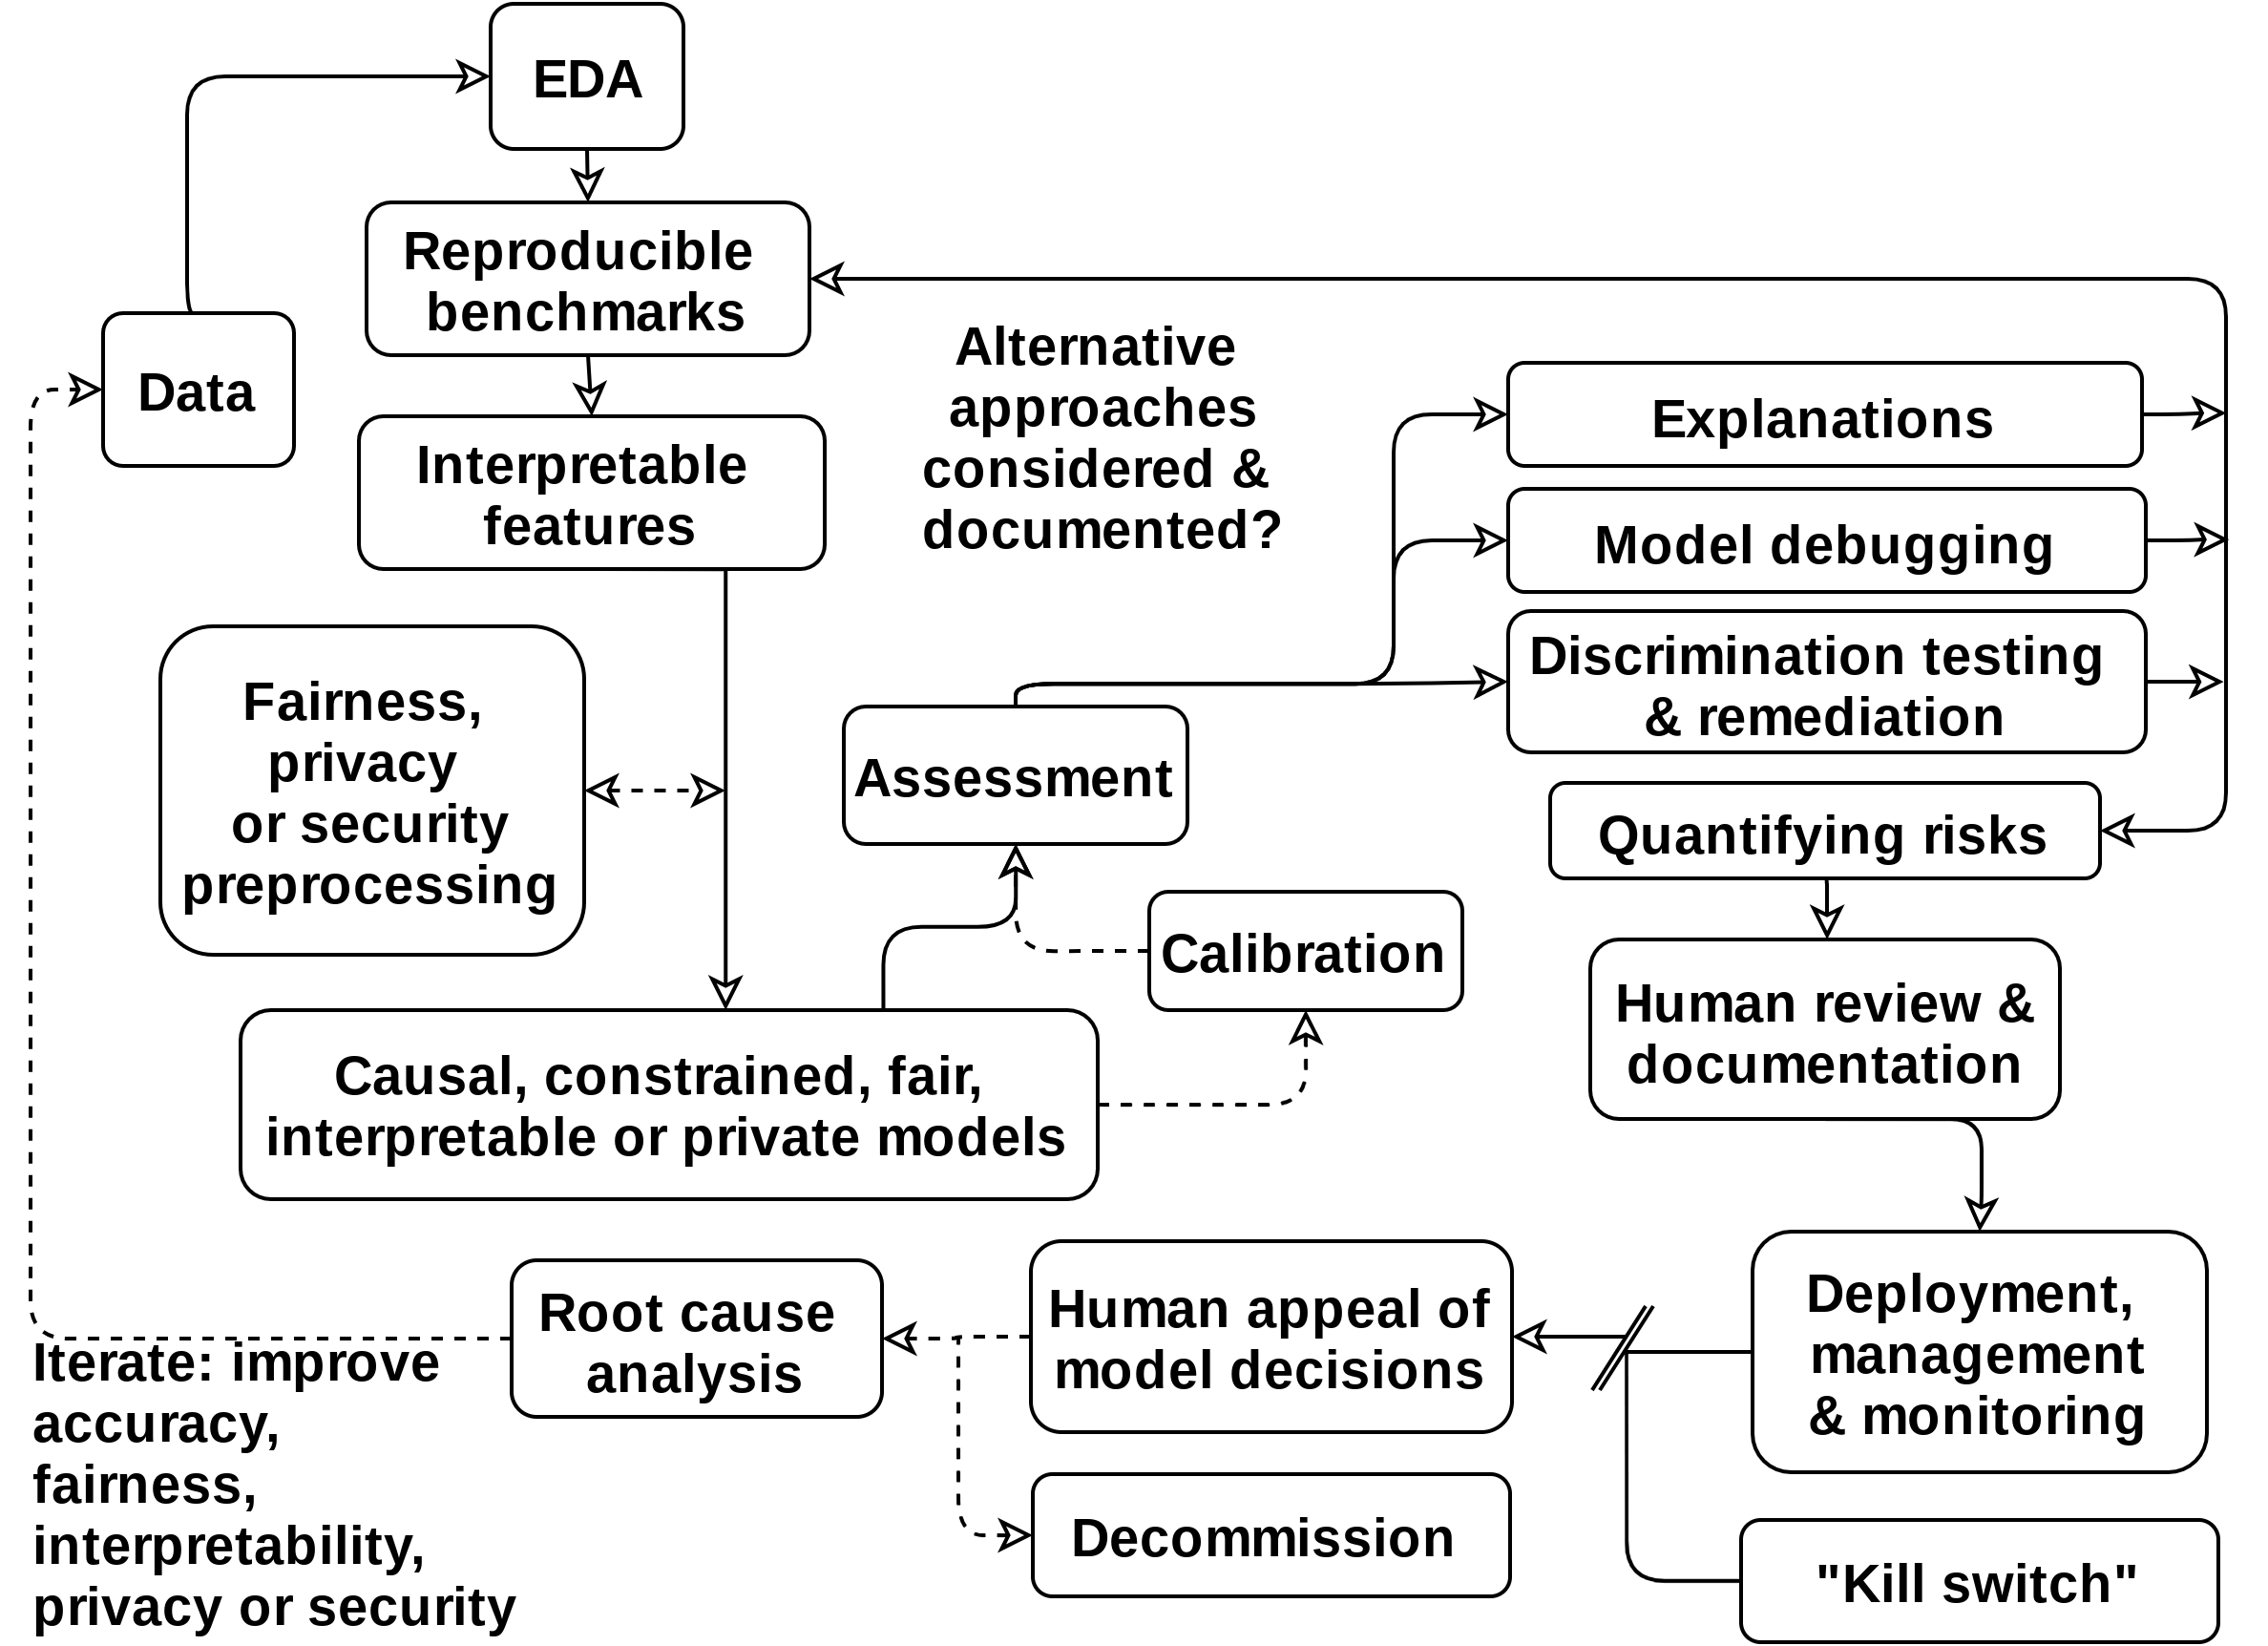
\includegraphics[height=150pt]{../img/rml_diagram_no_hilite.png}\\\vspace{5pt}
					\label{fig:blueprint_nohl}
					\scriptsize{\textbf{Source:} \href{https://www.mdpi.com/2078-2489/11/3/137/htm}{\textit{A Responsible Machine Learning Workflow}}.}
				\end{center}
			\end{figure}
		
		\end{frame}
		
		\begin{frame}
	
			\frametitle{A Responsible ML Workflow: Interpretable Models}		
			
			\begin{figure}[htb]
				\begin{center}
					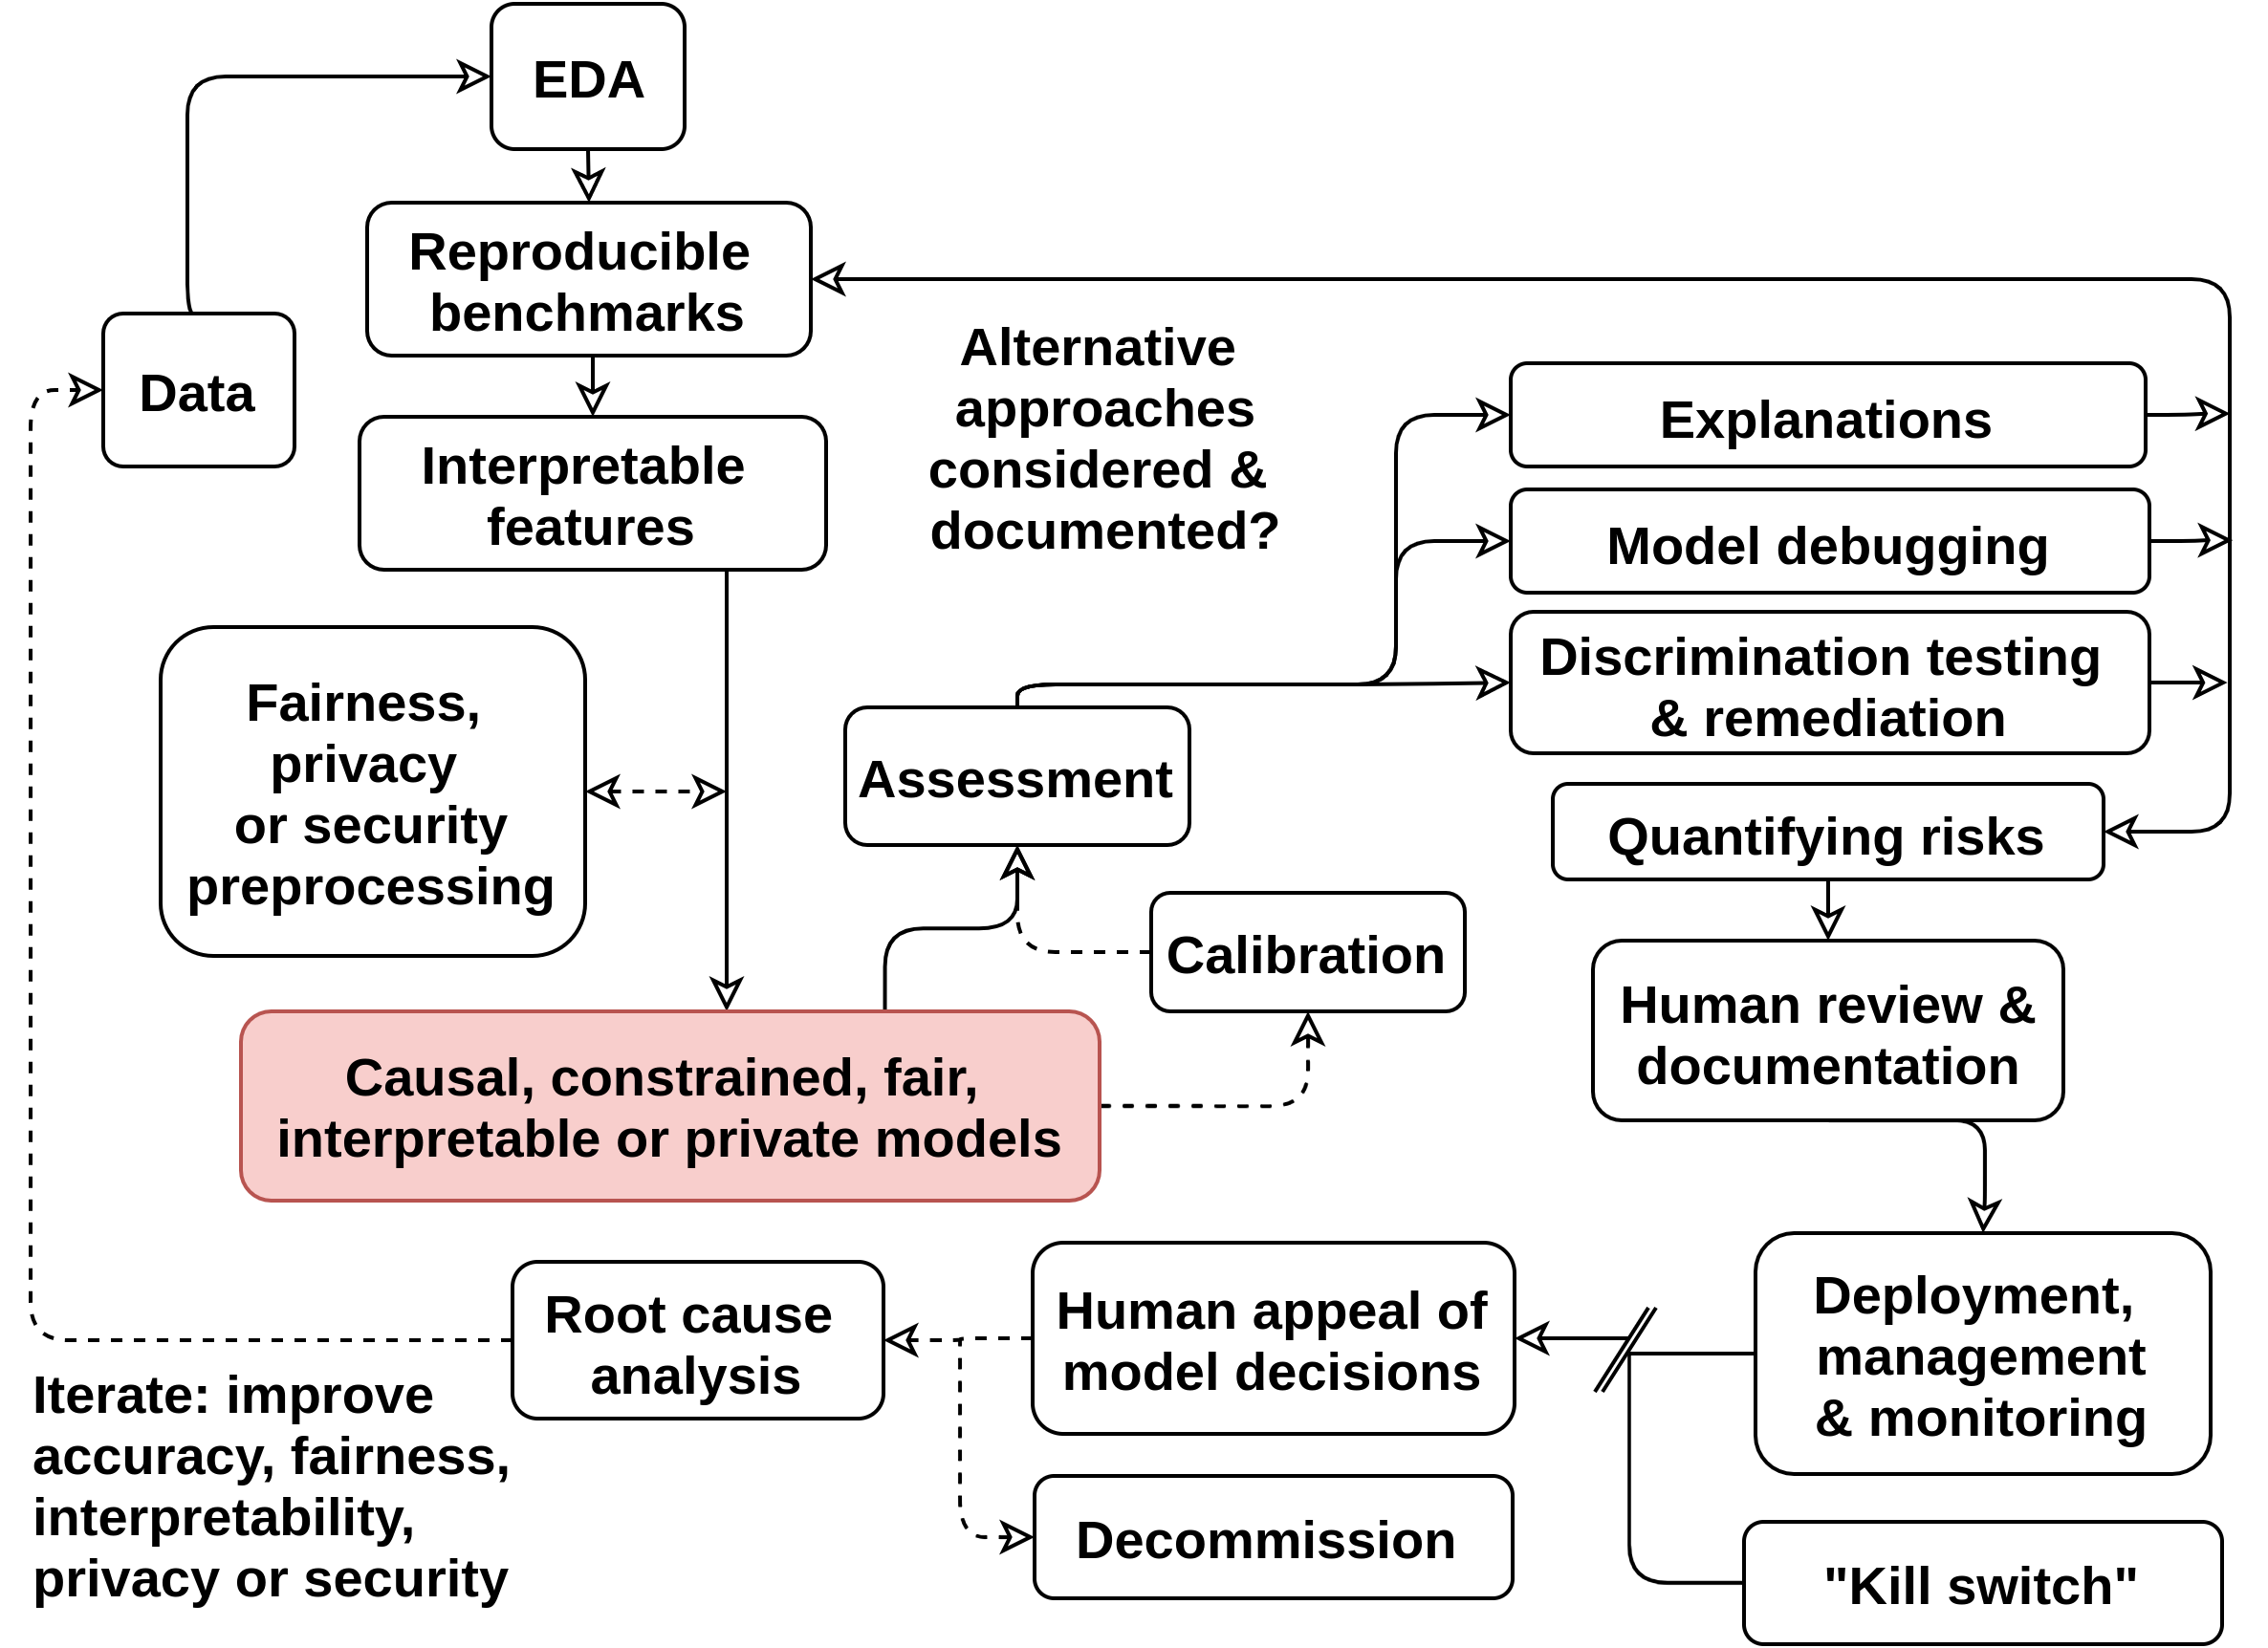
\includegraphics[height=150pt]{../img/rml_diagram_lec1_hilite.png}\\\vspace{5pt}
					\label{fig:blueprint_l1hl}
					\scriptsize{\textbf{Source:} \href{https://www.mdpi.com/2078-2489/11/3/137/htm}{\textit{A Responsible Machine Learning Workflow}}.}
				\end{center}
			\end{figure}		
					
		\end{frame}					

		\begin{frame}
	
			\frametitle{Interpretable ML Models}			
			
			\small
			
			\cite{been_kim1}, define interpretable as, ``the ability to explain or to present in understandable terms to a human.''
			
			\vspace{10pt}
			
			There are many types of interpretable ML models. Some might be directly interpretable to non-technical consumers. Some are only interpretable to highly-skilled data scientists. Interpretability is not an on-and-off switch.
			
			\vspace{10pt}
			
			Interpretable models are crucial for documentation, explanation of predictions to consumers, finding and fixing discrimination, and debugging other problems in ML modeling pipelines. Simply put, \textbf{it is very difficult to mitigate risks you don't understand}.
			
			\vspace{10pt}
			
			There is not necessarily a trade-off between accuracy and interpretability, especially for structured data.
			
			\normalsize
			
			
		\end{frame}	

		\begin{frame}
		
			\frametitle{Background}		
			
			We will frequently refer to the following terms and definitions today: \\			
			
			\begin{itemize}
				\item{Notation}
				\item{Pearson correlation}
					\begin{itemize}
						\item{Measurement of the linear relationship between two input $X_j$ features; takes on values between -1 and +1, including 0.}
					\end{itemize}
				\item{Shapley value}
				\item{Partial dependence and individual conditional expectation (ICE)}
				\item{Gradient boosting machine (GBM)}
			\end{itemize}			
		
		\end{frame}

		\begin{frame}[allowframebreaks]
	
			\frametitle{Background: Notation}
			
			\textbf{Spaces} 
			
			\begin{itemize}
				\item Input features come from the set $\mathcal{X}$ contained in a \textit{P}-dimensional input space, $\mathcal{X} \subset \mathbb{R}^P$.  An arbitrary, potentially unobserved, or future instance of $\mathcal{X}$ is denoted $\mathbf{x}$, $\mathbf{x} \in \mathcal{X}$.
				\item Labels corresponding to instances of $\mathcal{X}$ come from the set $\mathcal{Y}$.
				\item Learned output responses come from the set $\mathcal{\hat{Y}}$.
			\end{itemize}	
			
			\framebreak	
			
			\textbf{Datasets} 
			
			\begin{itemize}
				\item The input dataset $\mathbf{X}$ is composed of observed instances of the set $\mathcal{X}$ with a corresponding dataset of labels $\mathbf{Y}$, observed instances of the set $\mathcal{Y}$. 
				\item Each $i$-th observation of $\mathbf{X}$ is denoted as\\ $\mathbf{x}^{(i)} = $  
				$[x_0^{(i)}, x_1^{(i)}, \dots, x_{\textit{P}-1}^{(i)}]$, with corresponding $i$-th labels in $\mathbf{Y}, \mathbf{y}^{(i)}$, and corresponding predictions in $\mathbf{\hat{Y}}, \mathbf{\hat{y}}^{(i)}$.
				\item $\mathbf{X}$ and $\mathbf{Y}$ consist of $N$ tuples of observations:\\ $[(\mathbf{x}^{(0)},\mathbf{y}^{(0)}), (\mathbf{x}^{(1)},\mathbf{y}^{(1)}), \dots,(\mathbf{x}^{(N-1)},\mathbf{y}^{(N-1)})]$.
				\item Each $j$-th input column vector of $\mathbf{X}$ is denoted as $X_j = [x_{j}^{(0)}, x_{j}^{(1)}, \dots, x_{j}^{(N-1)}]^T$.
			\end{itemize}	 
			
			\framebreak
			
			\textbf{Models}
			
			\begin{itemize}
				\item A type of machine learning (ML) model $g$, selected from a hypothesis set $\mathcal{H}$, is trained to represent an unknown signal-generating function $f$ observed as  $\mathbf{X}$ with labels $\mathbf{Y}$ using a training algorithm $\mathcal{A}$: 
				$ \mathbf{X}, \mathbf{Y} \xrightarrow{\mathcal{A}} g$, such that $g \approx f$.
				\item $g$ generates learned output responses on the input dataset $g(\mathbf{X}) = \mathbf{\hat{Y}}$, and on the general input space $g(\mathcal{X}) = \mathcal{\hat{Y}}$.
				\item The model to be explained, tested for discrimination, or debugged is denoted as $g$.
			\end{itemize}
			
		\end{frame}

		\begin{frame}
		
			\frametitle{Background: Shapley Value}	
			
			Shapley explanations, including TreeSHAP and even certain implementations of LIME, are a class of additive, locally accurate feature contribution measures with long-standing theoretical support (\cite{shapley}). 

			\vspace{8pt}
			
			For some observation $\mathbf{x} \in \mathcal{X}$, Shapley explanations take the form:
			
			\begin{equation}
				\label{eq:shap_contrib}
				\begin{aligned}
					\phi_{j} = \underbrace{\sum_{S \subseteq \mathcal{P} \setminus \{j\}}\frac{|S|!(\mathcal{P} -|S| -1)!}{\mathcal{P}!}}_\text{weighted average over all subsets in \textbf{X}}\underbrace{[(S \cup \{j\}) - g_x(S)]}_{g\text{ "without" }x_j}
				\end{aligned}
			\end{equation}
			
			\begin{equation}
				\label{eq:shap_additive}
				\begin{aligned}
					g(\mathbf{x}) = \phi_0 + \sum_{j=0}^{j=\mathcal{P} - 1} \phi_j \mathbf{z}_j
				\end{aligned}
			\end{equation}
			
		\end{frame}
		
		\begin{frame}
		
			\frametitle{Background: Partial Dependence and ICE}			

			\begin{itemize}

			\item Following \citet{esl} a single input feature, $X_j \in \mathbf{X}$, and its complement set, $\mathbf{X}_{\mathcal{P} \setminus \{j\}} \in \mathbf{X}$, where $X_j \cup \mathbf{X}_{\mathcal{P} \setminus \{j\}} = \mathbf{X}$ is considered. $\text{PD}(X_j, g)$ for a given feature $X_j$ is estimated as the average output of the learned function $g(\mathbf{X})$ when all the components of $X_j$ are set to a constant $x \in \mathcal{X}$ and $\mathbf{X}_{(-j)}$ is left unchanged.

			\item $\text{ICE}(x_j, \mathbf{x}, g)$ for a given instance $\mathbf{x}$ and feature $x_j$ is estimated as the output of $g(\mathbf{x})$ when $x_j$ is set to a constant $x \in \mathcal{X}$ and all other features $\mathbf{x} \in \mathbf{X}_{(-j)}$ are left untouched. Partial dependence and ICE curves are usually plotted over some set of constants $x \in \mathcal{X}$ (\cite{ice_plots}). 

			\end{itemize} 			
					
		\end{frame}		
		
		\begin{frame}
		
			\frametitle{Background: Gradient Boosting Machine}			
				  			
			\begin{equation}
			\begin{aligned}\label{eq:gbm}
			g^{\text{GBM}}(\mathbf{x}) &= \sum_{b=0}^{B-1} T_b\left(\mathbf{x}; \Theta\right)
			\end{aligned}
			\end{equation}
			
			\vspace{20pt}
			
			A GBM is a sequential combination of decision trees, $T_b$, where $T_0$ is trained to predict $\mathbf{y}$, but all subsequent $T$ are trained to reduce the errors of $T_{b-1}$.
			
		\end{frame}	
					
%-------------------------------------------------------------------------------
	\section{Penalized GLM}
%-------------------------------------------------------------------------------
	
		\subsection*{}


		\begin{frame}
	
		\frametitle{Anatomy of Elastic Net Regression}	
				
		Generalized linear models (GLM) have the same basic functional form as more traditional linear models, e.g. ...
				
		\begin{equation}
			\begin{aligned}\label{eq:gbm}
			g^{\text{GLM}}(\mathbf{x}) &= \beta_0 + \beta_1 x_0 + \beta_2 x_1 + \dots + \beta_P x_{P-1}
			\end{aligned}
		\end{equation}	
		
		\vspace{10pt}... but are more robust to correlation, wide data, and outliers.
		
		\end{frame}

		\begin{frame}
		
			\frametitle{Anatomy of Elastic Net Regression: L1 and L2 Penalty}			
		Iteratively reweighted least squares (IRLS) method with ridge ($L_2$) and LASSO ($L_1$) penalty terms: 
			
			\begin{equation}
				\label{eq:Elastic_Net}
				\begin{aligned}
				\tilde{\beta}= \underset{\beta}{min}\Big\{ \mathcolorbox{red}{ \underbrace{\sum_{i=0}^{N-1}(y_i-\beta_0-\sum_{j=1}^{P-1} x_{ij} \beta_{j})^2}_\text{1}} + \mathcolorbox{red}{\underbrace{\lambda}_\text{2}} \sum_{j=1}^{P-1} ( \mathcolorbox{red}{\underbrace{\alpha}_\text{3}} \mathcolorbox{red}{\underbrace{\beta_j^2}_\text{4}} + (1-\mathcolorbox{red}{\underbrace{\alpha}_\text{3}}) \mathcolorbox{red}{\underbrace{|\beta_{j}|}_\text{5}}) \Big\}
				\end{aligned}
			\end{equation}		
			
			\begin{itemize}
			\scriptsize{
				\item{1: Least squares minimization}
				\item{2: Controls magnitude of penalties}
				\item{3: Tunes balance between L1 and L2}
				\item{4: $L_2$/Ridge penalty term}
				\item{5: $L_1$/LASSO penalty term}}
			\end{itemize}
						
		\end{frame}
	
		\begin{frame}
			
			\textbf{Graphical Illustration of Shrinkage/Regularization Method:} 
			
			\begin{figure}[htb]
				\begin{center}
					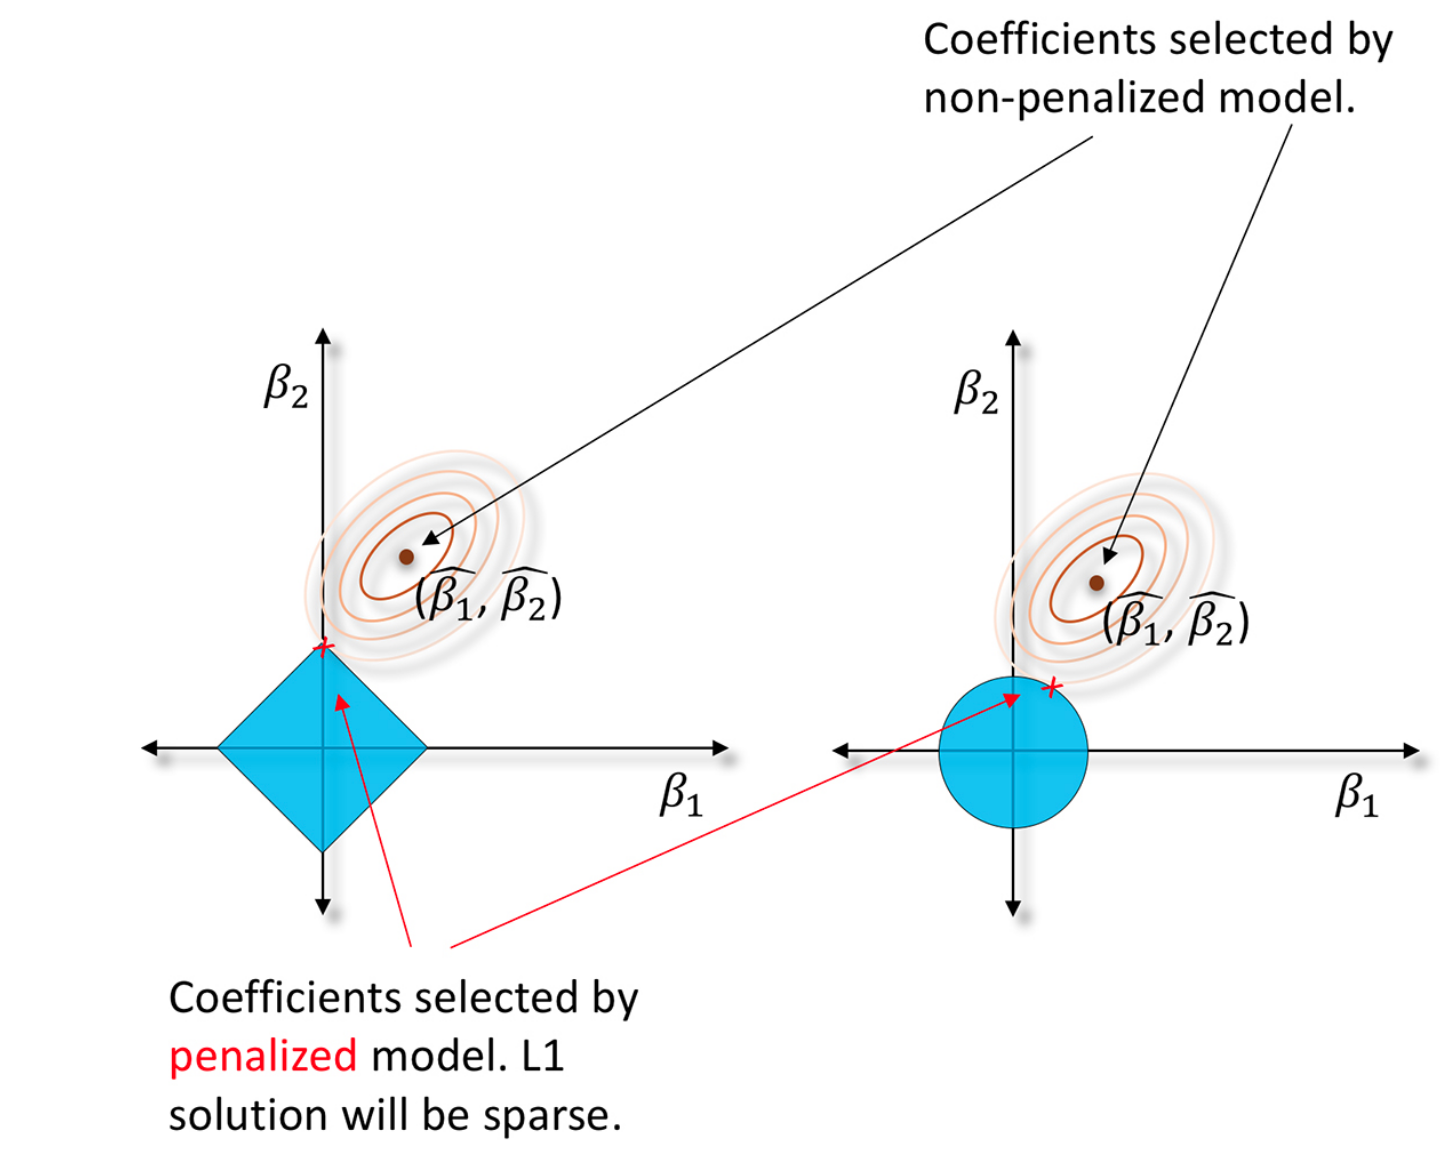
\includegraphics[height=150pt]{../img/L1L2_penalty_diagram.png}
					\label{fig:L1L2}
				\end{center}
			\end{figure}
								
		\end{frame}				
		
%-------------------------------------------------------------------------------
	\section{Monotonic GBM}
%-------------------------------------------------------------------------------

	\subsection*{}
	
	\begin{frame}
	
		\frametitle{Monotonic GBM (\cite{rml_workflow})}

			Monotonic GBM (MGBM) constrain typical GBM training to consider only tree splits that obey user-defined positive and negative monotone constraints, with respect to each input feature, $X_j$, and a target feature, $\mathbf{y}$, independently. An MGBM remains an additive combination of $B$ trees trained by gradient boosting, $T_b$, and each tree learns a set of splitting rules that respect monotone constraints,  $\Theta^\text{mono}_b$. A trained MGBM model, $g^{\text{MGBM}}$, takes the form:
			
			\begin{equation}
			\begin{aligned}\label{eq:gbm}
			g^{\text{MGBM}}(\mathbf{x}) &= \sum_{b=0}^{B-1} T_b\left(\mathbf{x}; \Theta^\text{mono}_b\right)
			\end{aligned}
			\end{equation}
		
	\end{frame}


	\begin{frame}
	
	\frametitle{Monotone Constraints for GBM (\cite{rml_workflow})}
	
		\begin{enumerate}\scriptsize
			\item For the first and highest split in $T_b$ involving $X_j$, any $\theta_{b,j,0}$ resulting in $T(x_j; \theta_{b,j,0}) = \{w_{b,j,0,L}, w_{b,j,0,R}\}$ where $w_{b,j,0,L} > w_{b,j,0,R}$, is not considered. 
			\item For any subsequent left child node involving $X_j$, any $\theta_{b,j, k\ge1}$ resulting in $T(x_j; \theta_{b,j,k\ge1}) = \{w_{b,j,k\ge1,L}, w_{b,j,k\ge1,R}\}$ where $w_{b,j,k\ge1,L} > w_{b,j,k\ge1,R}$, is not considered.
			\item Moreover, for any subsequent left child node involving $X_j$, $T(x_j; \theta_{b,j,k\ge1}) = \{w_{b,j,k\ge1,L}, w_{b,j,k\ge1,R}\}$, $\{w_{b,j,k\ge1,L}, w_{b,j,k\ge1,R}\}$ are bound by the associated $\theta_{b,j,k-1}$ set of node weights, $\{w_{b,j,k-1,L}, w_{b,j,k-1, R}\}$, such that $ \{w_{b,j,k\ge1,L}, w_{b,j,k\ge1,R}\} < \frac{w_{b,j,k-1,L} + w_{b,j,k-1,R}}{2}$.
			\item (1) and (2) are also applied to all right child nodes, except that for right child nodes $ w_{b,j,k,L} \le w_{b,j,k,R}$ and $\{w_{b,j,k\ge1,L}, w_{b,j,k\ge1,R}\} \ge \frac{w_{b,j,k-1,L} + w_{b,j,k-1,R}}{2}$.
		\end{enumerate}
	
	Note that $g^{\text{MGBM}}(\mathbf{x})$ is an addition of each full $T_b$ prediction, with the application of a monotonic logit or softmax link function for classification problems. Moreover, each tree's root node corresponds to some constant node weight that by definition obeys monotonicity constraints, $ T(x^{\alpha}_j; \theta_{b,0}) = T(x^{\beta}_j; \theta_{b,0}) = w_{b,0}$. 
	
	\end{frame}

	\begin{frame}
	
			\textbf{Partial Dependence and ICE:}

			\begin{figure}[htb]
				\begin{center}
					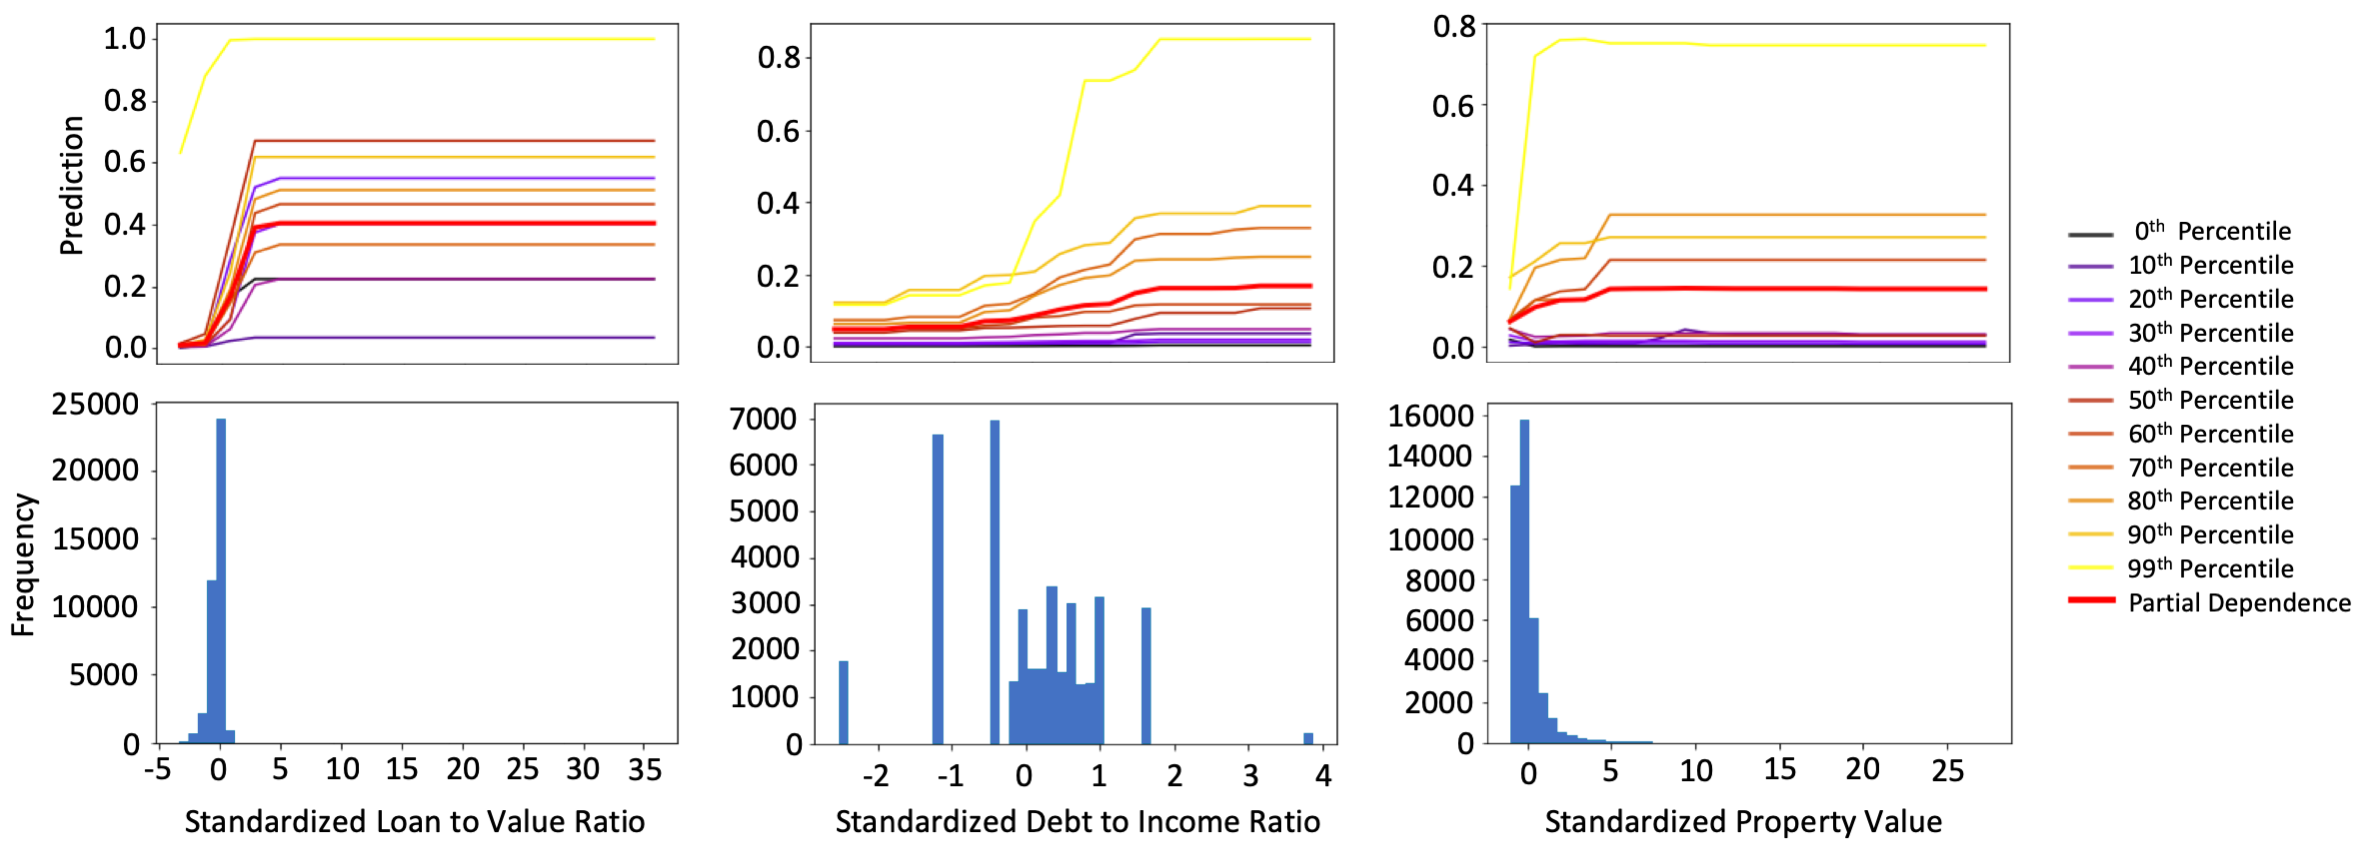
\includegraphics[height=150pt]{../img/mort_mgbm_glob_pdp_ice.png}
					\label{fig:mgbm}
				\end{center}
			\end{figure}
	
	\end{frame}



%-------------------------------------------------------------------------------
	\section{A Burgeoning Ecosystem}
%--------------------------------------------------------------------------
			
		\subsection*{}
		
		\begin{frame}
		
			\frametitle{A Burgeoning Ecosystem of Interpretable Machine Learning Models}		
			
			\begin{itemize}
				\item \href{https://www.r-bloggers.com/generalized-additive-models}{Generalized additive model} (GAM) (\cite{esl})
				\item \href{http://www.cs.cornell.edu/~yinlou/projects/gam/}{GA2M} / \href{https://github.com/interpretml/interpret/}{Explainable boosting machine} (EBM) (\cite{ga2m})
				\item \href{https://www.mdpi.com/2078-2489/11/3/137}{Explainable Neural Network} (XNN) (\cite{wf_xnn})
				\item Rudin group: 
				\begin{itemize}
					\item \href{https://www.youtube.com/watch?v=k3IQnRsl9U4}{\textit{This looks like that} deep learning} (\cite{this_looks_like_that})
					\item Scalable Bayesian rule list (\cite{sbrl}) 
					\item Optimal sparse decision tree (\cite{osdt})
					\item Supersparse linear integer models (\cite{slim})
					\item and more ... 
				\end{itemize}
				\item \href{https://christophm.github.io/interpretable-ml-book/rulefit.html}{RuleFit} (\cite{rulefit})
			\end{itemize}
		
		\end{frame}
		
%-------------------------------------------------------------------------------
\section{Acknowledgments}
%--------------------------------------------------------------------------

\subsection*{}

\begin{frame}[t]
	
	\frametitle{Acknowledgments}		
	
	Thanks to Lisa Song for her continued assistance in developing these course materials.\\
	\vspace{10pt}
	Some materials \copyright\hspace{1pt}Patrick Hall and the H2O.ai team 2017-2020. 
	
	
	
\end{frame}
		
%-------------------------------------------------------------------------------
%	References
%-------------------------------------------------------------------------------

	\begin{frame}[t, allowframebreaks]
	
		\frametitle{References}	
		
		\printbibliography
		
	\end{frame}

\end{document}
